\documentclass[12pt,a4paper]{article}
\usepackage{multirow}
\usepackage{rotating}
\usepackage{graphicx}
\usepackage{amsmath}
\usepackage{amsfonts}
\usepackage{amssymb}
\usepackage{graphicx}
\pagestyle{empty}
%\usepackage[bottom=0.5in,headheight=0pt,headsep=0pt]{geometry}
%\addtolength{\topmargin}{0pt}
\usepackage{xepersian}
\linespread{1.2}
\settextfont{XB Niloofar}

\begin{document}
\begin{center}
	بسمه تعالی
\end{center}
\begin{center}
	\textbf{
		پاسخ سری سوم تمرین‌ها
		- درس ریاضیات گسسته - دانشگاه صنعتی شریف}
	\\
	علیرضا توفیقی محمدی - رشته علوم کامپیوتر - شماره‌دانشجویی: ۹۶۱۰۰۳۶۳
\end{center}
\section{تمرین ششم}
\subsubsection{صورت سوال}
برای اعداد طبیعی 
$m \leq n$
فرمول بسته‌ی 
$\sum_{k=m}^n \binom{k}{m}\binom{n}{k}$
را حساب کنید.
\subsubsection{پاسخ}
به‌شکل ترکیبیاتی ثابت می‌کنیم 
\[
\sum_{k=m}^n \binom{k}{m}\binom{n}{k} = \binom{n}{m}\times 2^{n-m}
\]
برای اینکار مسئله‌ی شمارشی زیر را مطرح می‌کنیم:
\\
می‌خواهیم از مجموعه‌ی 
$\{1,..., n\}$
یک زیرمجموعه‌ انتخاب کرده و سپس دقیقا $m$ تا از اعضایش را رنگی کنیم. برای اینکار چند حالت داریم.
\\
از طرفی برای اینکار می‌توانیم ابتدا $m$ عضو رنگی را انتخاب کرده که برای اینکار 
$\binom{n}{m}$
روش داریم، سپس از $n-m$ عضو دیگر، یک زیرمجموعه انتخاب کرده و با $m$ عضو انتخاب‌شده‌ی قبل به عنوان مجموعه ارائه دهیم که برای اینکار نیز 
$2^{n-m}$
روش داریم پس در کل طبق اصل ضرب 
$\binom{n}{m} 2^{n-m}$
روش داریم.
\\
از طرف دیگر فرض کنید مجموعه‌ی ما $k$ عضو داشته باشد 
$(k \in \{m, ..., n\})$
.
برای انتخاب مجموعه 
$\binom{n}{k}$
حالت و برای انتخاب اعضای رنگی آن
$\binom{k}{m}$
حالت داریم پس با فرض ثابت بودن $k$ برای این حالت
$\binom{k}{m}\binom{n}{k}$
حالت داریم.
\\
پس طبق اصل جمع کل حالت‌ها برابر با 
$\sum_{k=m}^n \binom{k}{m}\binom{n}{k}$
است.

\section{تمرین هفتم}
\subsection{قسمت الف}
\subsubsection{صورت سوال}
فرمول بسته‌ی 
$\sum_{k=1}^n \binom{k}{m}\frac{1}{k}$
را حساب کنید.
\subsubsection{پاسخ}
برای حل مسئله ابتدا سعی می‌کنیم
$\binom{k}{m}\frac{1}{k}$
را به شکلی ساده‌تر بنویسیم:
\[
\binom{k}{m}\frac{1}{k} = \frac{k!}{m!(k-m)!k} = \frac{(k-1)!}{(m-1)!(k-m)!m}
= \binom{k-1}{m-1}\frac{1}{m}
\]
حال به حل مسئله‌ی اصلی می‌پردازیم:
\[
\sum_{k=1}^n \binom{k}{m}\frac{1}{k} = \sum_{k=1}^n \binom{k-1}{m-1}\frac{1}{m}
= \frac{\sum_{k=0}^{n-1} \binom{k}{m-1}}{m} 
= \frac{\binom{n}{m}}{m}
\]
و مسئله حل شد.
\subsection{قسمت ب}
\subsubsection{صورت سوال}
فرمول بسته‌ی 
$\sum_{k=0}^n \binom{k}{m}k$
را حساب کنید.
\subsubsection{پاسخ}
با نوشتن عبارت بالا به صورت دو سیگمای تودرتو سعی بر حل عبارت می‌کنیم:
\[
\sum_{k=0}^n \binom{k}{m}k = \sum_{k=1}^n \binom{k}{m}k = \sum_{i=1}^n \sum_{k=i}^{n} \binom{k}{m}
= \sum_{i=1}^n\left( \sum_{k=0}^n \binom{k}{m} - \sum_{k=0}^{i-1} \binom{k}{m}\right)
\]
\[
= \sum_{i=1}^n\left( \binom{n+1}{m+1} - \binom{i}{m+1}\right)
= n\binom{n+1}{m+1} - \binom{n+1}{m+1} + \binom{0}{m+1}
\]
\[
= (n-1)\binom{n+1}{m+1}
\]

\section{تمرین هشتم}
\subsection{صورت سوال}
ثابت کنید
$n! \leq \sqrt{n}e \left(\frac{n}{e}\right)^n$
\subsection{پاسخ}
همانند اثبات قضیه پیش می‌رویم با این تفاوت که مقدار 
مثلث‌های رنگی شکل ۱ را نیز از انتگرال کم می‌کنیم:
\begin{figure}
	\centering
	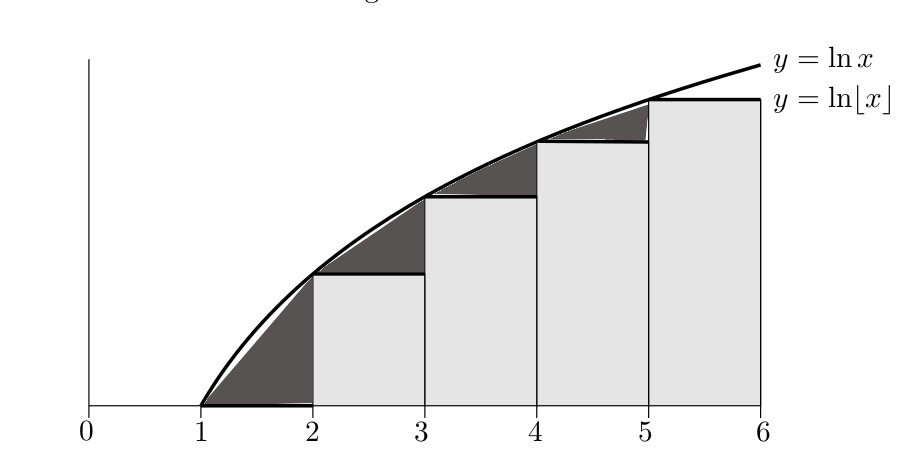
\includegraphics[width=0.7\linewidth]{1}
	\caption{نمودار $\ln x$ و مثلث‌هایی که باید از انتگرال‌ها کم کنیم}
	\label{fig:1}
\end{figure}
حال به محاسبه‌ی $\ln n!$ می‌پردازیم:
\[
\ln n! = \sum_{i=1}^{n} \ln n 
\leq \left(\sum_{i=1}^{n-1}\left(\int_{i}^{i+1}\ln x  dx - \frac{\ln(i+1)-\ln(i)}{2} \right)\right) + \ln n
\]
\[
= \int_{i=1}^n \ln x dx - \frac{\ln(n)}{2} + \ln n
= (n+1)\ln n - n + 1 - \frac{\ln n}{2}
\]
\[
\rightarrow n! \leq \frac{n^{(n+1)}\times e}{e^n \times \sqrt{n}}
= \sqrt{n}e \left(\frac{n}{e}\right)^n
\]
و حکم ثابت شد.

\end{document}